\begin{frame}
  \myheading{Module 6.2 : Linear Algebra - Basic Definitions}
\end{frame}

% Slide 10
\begin{frame}
  \begin{itemize}\justifying
    \item We will see some more examples where eigenvectors are important, but before that let's revisit some basic definitions from linear algebra.
  \end{itemize}

\end{frame}

% Slide 11
\begin{frame}
  \begin{overlayarea}{\textwidth}{\textheight}
    \only<1->{
      \begin{block}{Basis}
        A set of vectors $\in \mathbb{R}^n$ is called a basis, if they are \underline{linearly
          independent} and every vector $\in \mathbb{R}^n$ can be expressed as a linear combination of
        these vectors.
      \end{block}
    }
    \only<2->{
      \begin{block}{Linearly independent vectors}
        A set of $n$ vectors $v_1, v_2, \dots, v_n$ is linearly independent if no vector in the
        set can be expressed as a linear combination of the remaining $n-1$ vectors.
        \newline
        In other words, the only solution to
        \[
          c_1v_1 + c_2v_2 + \dots c_nv_n = 0 \textrm{ is } c_1 = c_2 = \dots = c_n = 0 (\textit{$c_i$'s are scalars})
        \]
      \end{block}
    }
  \end{overlayarea}
\end{frame}

% Slide 12
\begin{frame}
  \begin{columns}
    \column{0.4\textwidth}
    \begin{overlayarea}{\textwidth}{\textheight}
      \begin{center}
        \begin{tikzpicture}[scale=1]
  \draw [thick, black, ->] (0,0) -- (4, 0);
  \draw [thick, red, ->] (0,0) -- (1,0)
  node [below, black] {$x = (1,0)$};
  \draw [thick, black, ->] (0,0) -- (0, 4);
  \draw [thick, red, ->] (0,0) -- (0, 1)
  node [left, black] {$y = (0,1)$};
\end{tikzpicture}

      \end{center}
    \end{overlayarea}

    \column{0.6\textwidth}
    \begin{overlayarea}{\textwidth}{\textheight}
      \only<1->{
        \begin{itemize}\justifying
          \item<1-> For example consider the space $\mathbb{R}^2$
          \item<2-> Now consider the vectors
                \[x = \left[ \begin{array}{c}
                      1 \\
                      0
                    \end{array} \right] \text{ and }
                  y = \left[ \begin{array}{c}
                      0 \\
                      1
                    \end{array} \right]
                \]
          \item<3-> Any vector $\left[ \begin{array}{c}
                      a \\
                      b
                    \end{array} \right] \in \mathbb{R}^2$, can be expressed as
                a linear combination of these two vectors i.e
                \[\left[ \begin{array}{c}
                      a \\
                      b
                    \end{array} \right] =
                  a \left[ \begin{array}{c}
                      1 \\
                      0
                    \end{array} \right] +
                  b \left[ \begin{array}{c}
                      0 \\
                      1
                    \end{array} \right]
                \]
          \item<4-> Further, $x$ and $y$ are linearly independent.
                \newline
                (the only solution to $c_1x + c_2y = 0$ is $c_1=c_2=0$)
        \end{itemize}
      }
    \end{overlayarea}
  \end{columns}
\end{frame}

% Slide 13
\begin{frame}
  \begin{columns}
    \column{0.4\textwidth}
    \begin{overlayarea}{\textwidth}{\textheight}
      \begin{center}
        \begin{tikzpicture}[scale=1]
  \draw [thick, black, ->] (0,0) -- (4, 0);
  \draw [thick, red, ->] (0,0) -- (1,0)
  node [below, black] {$x = (1,0)$};
  \draw [thick, black, ->] (0,0) -- (0, 4);
  \draw [thick, red, ->] (0,0) -- (0, 1)
  node [left, black] {$y = (0,1)$};
\end{tikzpicture}

        \vspace{0.2mm}
        \begin{align*}
        	\only<6-7>{\begin{bmatrix}a\\b\end{bmatrix} &= x_1 \begin{bmatrix}2\\3\end{bmatrix} + x_2 \begin{bmatrix}5\\7\end{bmatrix}\\}
        	\only<8->{a &= 2 x_1 + 5 x_2\\}
        	\only<8->{b &= 3 x_1 + 7 x_2\\}
        \end{align*}
      \end{center}
    \end{overlayarea}

    \column{0.6\textwidth}
    \begin{overlayarea}{\textwidth}{\textheight}
      \only<1->{
        \begin{itemize}\justifying
          \item<1-> In fact, turns out that $x$ and $y$ are unit vectors in the
                direction of the co-ordinate axes.
          \item<2-> And indeed we are used to representing all vectors in $\mathbb{R}^2$
                as a linear combination of these two vectors.
          \item<3-> But there is nothing sacrosanct about the particular choice of $x$ and $y$.
          \item<4-> We could have chosen any $2$ linearly independent vectors in $\mathbb{R}^2$
                as the basis vectors.
          \item<5-> For example, consider the linearly independent vectors, $[2,3]^T$ and $[5,7]^T$.
                See how any vector $[a,b]^T \in \mathbb{R}^2$ can be expressed as a linear combination of
                these two vectors.
          \item<7-> We can find $x_1$ and $x_2$ by solving a system of linear equations.
                % \newline
                % (Hint: Think simultaneous linear equations)
        \end{itemize}
      }
    \end{overlayarea}
  \end{columns}
\end{frame}

% Slide 14
\begin{frame}
  \begin{columns}
    \column{0.4\textwidth}
    \begin{overlayarea}{\textwidth}{\textheight}
      \only<1->{
        \begin{center}
          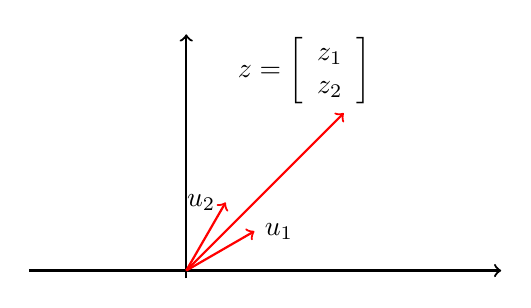
\begin{tikzpicture}[scale=1]
  \draw [thick, black, ->] (-2,0) -- (4, 0);
  \draw [thick, red, ->] (0,0) -- (0.866,0.5)
  node [right, black] {$u_1$};
  \draw [thick, black, ->] (0,-0.1) -- (0, 3);
  \draw [thick, red, ->] (0,0) -- (0.5, 0.866)
  node [left, black] {$u_2$};
  \draw [thick, red, ->] (0,0) -- (2,2);
  \draw (1.5,2)
  node [above] {$
      z = \left[ \begin{array}{c}
          z_1 \\
          z_2
        \end{array} \right]
    $};
\end{tikzpicture}

        \end{center}
      }
    \end{overlayarea}


    \column{0.6\textwidth}
    \only<1->{
      \begin{overlayarea}{\textwidth}{\textheight}
        \vspace{-0.2cm}
        \begin{itemize}\justifying
          \item<1-> In general, given a set of linearly independent vectors
                $u_1, u_2, \dots u_n \in \mathbb{R}^n$, we can express any vector
                $z \in \mathbb{R}^n$ as a linear combination of these vectors.
                \vspace{-0.3cm}
                \begin{align*}
                  \visible<2-> {z &= \alpha_1 u_1 + \alpha_2 u_2 + \dots + \alpha_n u_n}\\
                  \visible<3->{\begin{bmatrix}z_1\\z_2\\ \vdots \\z_n\end{bmatrix}
                                         &= \alpha_1 \begin{bmatrix}u_{11}\\u_{12}\\ \vdots \\u_{1n}\end{bmatrix}
                                            + \alpha_2 \begin{bmatrix}u_{21}\\u_{22}\\ \vdots \\u_{2n}\end{bmatrix}
                                            + \hdots
                                            + \alpha_n \begin{bmatrix}u_{n1}\\u_{n2}\\ \vdots \\u_{nn}\end{bmatrix}}\\
                   \visible<4->{\begin{bmatrix}z_1\\z_2\\ \vdots \\z_n\end{bmatrix} &= 
                                           \begin{bmatrix}
                                           	u_{11} & u_{21} & \hdots & u_{n1} \\
                                           	u_{12} & u_{22} & \hdots & u_{n2} \\
                                           	\vdots & \vdots & \vdots & \vdots \\
                                           	u_{1n} & u_{2n} & \hdots & u_{nn} \\
                                           \end{bmatrix}
                                           \begin{bmatrix} \alpha_1 \\ \alpha_2 \\ \vdots \\ \alpha_n\end{bmatrix} }
                \end{align*}
                \only<4>{ (Basically rewriting in matrix form)}
           \vspace{-0.4cm}
          \item<5-> We can now find the $\alpha_i$s using Gaussian Elimination (Time Complexity: $O(n^3)$)
        \end{itemize}
      \end{overlayarea}
    }
  \end{columns}
\end{frame}


% Slide 14
\begin{frame}
  \begin{columns}
    \column{0.4\textwidth}
    \begin{overlayarea}{\textwidth}{\textheight}
      \only<1->{
        \begin{center}
          \begin{tikzpicture}[scale=1]
  \draw [thick, black, ->] (-2,0) -- (4, 0);
  \draw [thick, red, ->] (0,0) -- (0.866,0.5)
  node [above, black] {$u_1$};
  \draw [thick, black, ->] (0,-0.1) -- (0, 3);
  \draw [thick, red, ->] (0,0) -- (-0.4,0.6928);
  \draw (-0.6, 0.75)
  node [above] {$u_2$};
  \draw [thick, red, ->] (0,0) -- (1,1.732);
  \draw (1.5,2)
  node [above] {$
      z = \left[ \begin{array}{c}
          a \\
          b
        \end{array} \right]
    $};
  \draw [dotted, black] (0.866,0.5) -- (1.5,0.866);
  \draw [dotted, black] (-0.25,0.433) -- (-0.5, 0.866);
  \draw [dotted, black] (1,1.732) -- (1.5,0.866);
  \draw [dotted, black] (-0.5, 0.866) -- (1,1.732);
  \draw (0.25,.144) arc (30:60:.32cm);
  \draw (0.35,.144)
  node [above, black] {$\theta$};
  \node [rotate=60] at (0.3,1.25) {$ |\overset{\rightarrow}{z}| $};
  \node [rotate=30] at (1,0.166) {$\alpha_1$};
  \node [rotate=120] at (-0.4, 0.066) {$\alpha_2$};
  \draw [decorate, decoration={brace, raise=3pt, mirror}] (0,0) -- (1.5, 0.866);
  \draw [decorate, decoration={brace, raise=3pt}] (0,0) -- (-0.5, 0.866);
\end{tikzpicture}

        \end{center}
      }
      \vspace{-0.5cm}
      \only<8->{
        \begin{align*}
          \alpha_1 = |\overset{\rightarrow}{z}| cos \theta
          = |\overset{\rightarrow}{z}| \frac{z^T u_1}{|\overset{\rightarrow}{z}| |u_1|} = z^T u_1
        \end{align*}
      }
      \only<9->{
        Similarly, $\alpha_2 = z^T u_2$. \newline
      }
      \only<10->{
        When $u_1$ and $u_2$ are unit vectors along the co-ordinate axes
        \vspace{-0.1in}
        \[
          z = \left[ \begin{array}{c}
              a \\
              b
            \end{array} \right]
          = a \left[ \begin{array}{c}
              1 \\
              0
            \end{array} \right]  +
          b \left[ \begin{array}{c}
              0 \\
              1
            \end{array} \right]
        \]
      }
    \end{overlayarea}


    \column{0.6\textwidth}
      \begin{overlayarea}{\textwidth}{\textheight}
        \vspace{-0.2cm}
        \begin{itemize}\justifying
        	\item<1-> Now let us see if we have orthonormal basis.
        	\item<2-> $u_i^T u_j = 0~\forall i\neq j$ and $u_i^T u_i = \|u_i\|^2 = 1$
        	\item<3-> Again we have:
        		\begin{align*}
        			\visible<3->{z &= \alpha_1 u_1 + \alpha_2 u_2 + \hdots + \alpha_n u_n\\}
        			\visible<4->{u_1^T z &=  \alpha_1 u_1^T u_1 + \hdots + \alpha_n u_1^T u_n\\}
        			\visible<5->{		&= \alpha_1}
        		\end{align*}
        	\item<6-> We can directly find each $\alpha_i$ using a dot product between $z$ and $u_i$ (time complexity $O(N)$)
        	\item<7-> The total complexity will be $O(N^2)$
        \end{itemize}
      \end{overlayarea}
  \end{columns}
\end{frame}

% Slide 15
\begin{frame}
  \begin{block}{Remember}
    An orthogonal basis is the most convenient basis that one can hope for.
  \end{block}
\end{frame}

% Slide 16
\begin{frame}
  \begin{columns}
    \column{0.4\textwidth}
    \begin{overlayarea}{\textwidth}{\textheight}
      \only<3->{
        \begin{block}{Theorem 1}
          The eigenvectors of a matrix $A \in \mathbb{R}^{n \times n}$ having distinct eigenvalues
          are linearly independent.
          \newline
          \textbf{Proof:} \href{https://math.stackexchange.com/questions/29371/how-to-prove-that-eigenvectors-from-different-eigenvalues-are-linearly-independe}{See here}
        \end{block}
      }
      \only<5->{
        \begin{block}{Theorem 2}
          The eigenvectors of a square symmetric matrix are orthogonal.
          \newline
          \textbf{Proof:} \href{https://math.stackexchange.com/questions/82467/eigenvectors-of-real-symmetric-matrices-are-orthogonal}{See here}
        \end{block}
      }
    \end{overlayarea}
    \column{0.6\textwidth}
    \begin{overlayarea}{\textwidth}{\textheight}
      \only<1->{
        \begin{itemize}\justifying
          \item<1-> But what does any of this have to do with eigenvectors?
          \item<2-> Turns out that the eigenvectors can form a basis.
          \item<4-> In fact, the eigenvectors of a square symmetric matrix are
                even more special.

          \item<6-> Thus they form a very convenient basis.
          \item<7-> Why would we want to use the eigenvectors as a basis instead
                of the more natural co-ordinate axes?
          \item<8-> We will answer this question soon.
        \end{itemize}
      }
    \end{overlayarea}
  \end{columns}
\end{frame}
